
%(BEGIN_QUESTION)
% Copyright 2006, Tony R. Kuphaldt, released under the Creative Commons Attribution License (v 1.0)
% This means you may do almost anything with this work of mine, so long as you give me proper credit

Draw a control circuit for the electric motor of an air compressor, controlled by two pressure switches: one switch turns the motor on when the pressure falls to 80 PSI, while the other switch turns the motor off when the pressure rises to 105 PSI:

%$$\includegraphics[width=15.5cm]{i00799x01.eps}$$

Be sure to include the overload (OL) contact in the 220 volt control circuit (L1 \& L2), and include a manual on/off switch as well.

\underbar{file i00799}
%(END_QUESTION)





%(BEGIN_ANSWER)

$$\includegraphics[width=15.5cm]{i00799x02.eps}$$

%(END_ANSWER)





%(BEGIN_NOTES)


%INDEX% Switch, pressure: ladder logic circuit

%(END_NOTES)


